\section{Actividad 5}

\subsection*{En el trabajo práctico anterior se analizó espectralmente una señal compuesta por tres 
sinusoides de frecuencias 50 Hz, 120 Hz y 200 Hz, con diferentes amplitudes y fases 
(constantes).}

\subsection*{a) Graficar la señal total en el dominio del tiempo y en el dominio de la frecuencia 
(mediante la Transformada Rápida de Fourier, FFT).} 

La señal total del práctico anterior es la siguiente:

\[
      \begin{aligned}
            x(t) &= 1.0 \cos\!\bigl(2\pi 50 t\bigr)
                  + 0.5 \cos\!\bigl(2\pi 120 t\bigr)
                  + 0.3 \cos\!\bigl(2\pi 200 t\bigr)
      \end{aligned}
\]

\bigskip
      \begin{figure}[H]
            \centering
            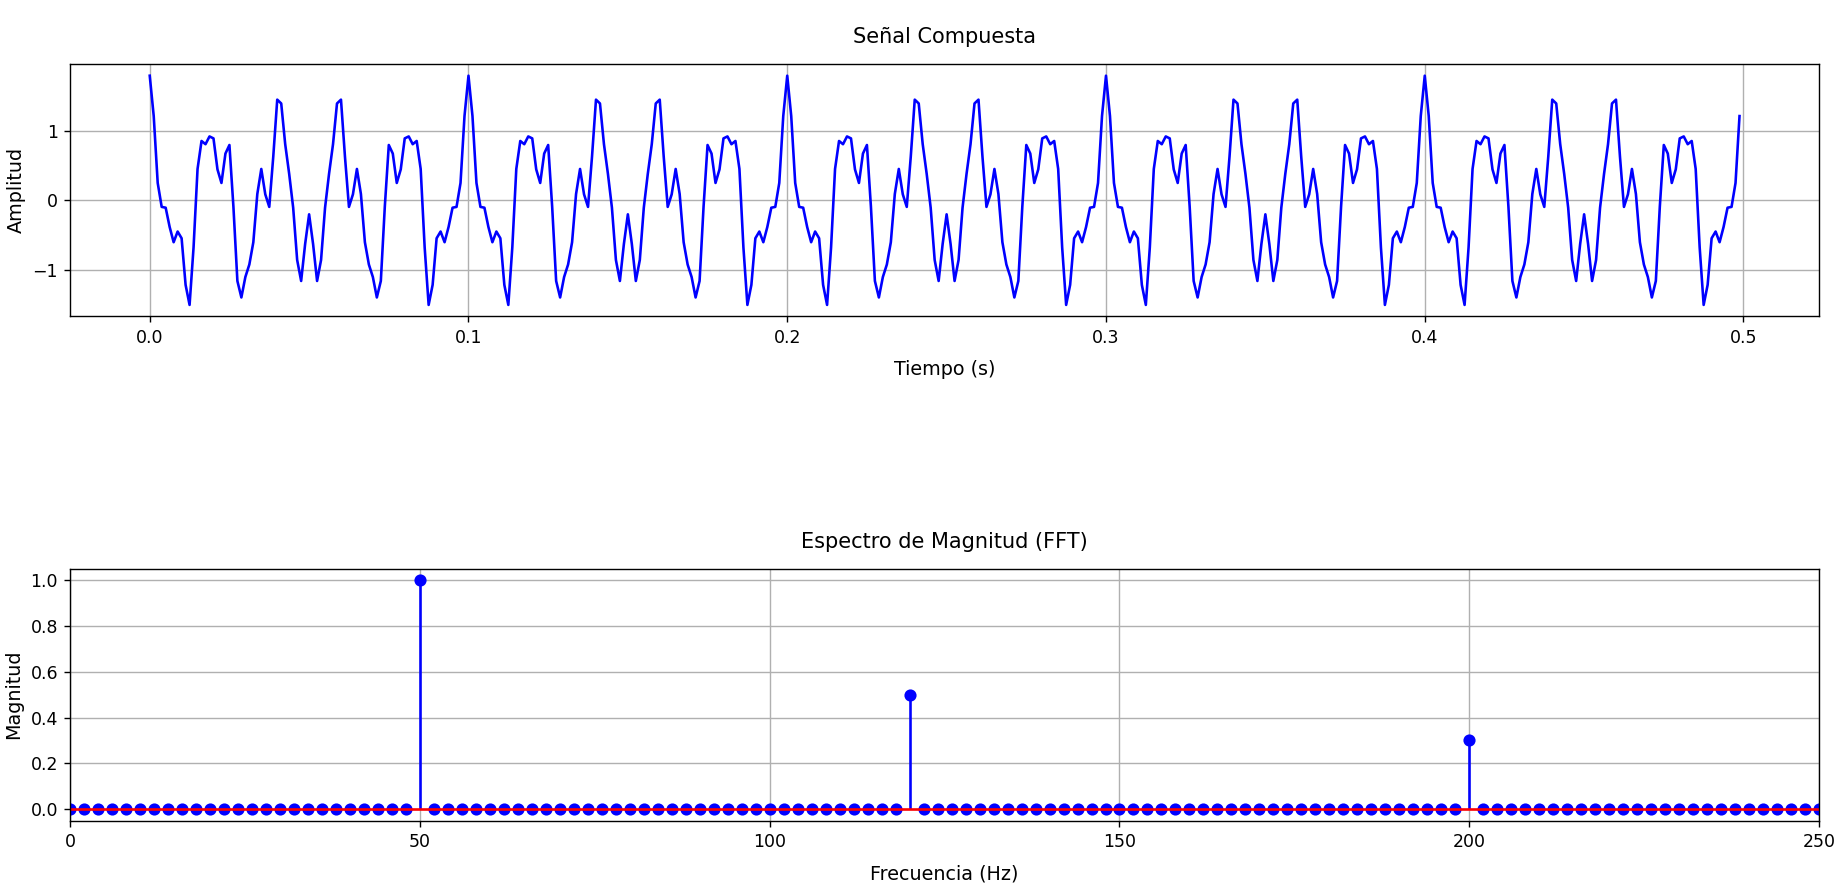
\includegraphics[width=0.8\textwidth]{imagenes/Actividad_5/senalcompuesta.png}
            \caption{Señal total.}
      \end{figure}
\bigskip

\subsection*{b) Incorporar a la señal ruido blanco gaussiano en dos escenarios:}

\begin{itemize}
    \item Ruido bajo: el nivel de ruido no es suficiente para ocultar las componentes sinusoidales.
    \item Ruido alto: el nivel de ruido es suficiente para enmascarar las componentes de la señal.
\end{itemize}

Para cada caso, representar nuevamente la señal tanto en el tiempo como en el espectro de frecuencias y analizar cómo varían la 
visibilidad de las componentes espectrales. \par

\bigskip
      \begin{figure}[H]
            \centering
            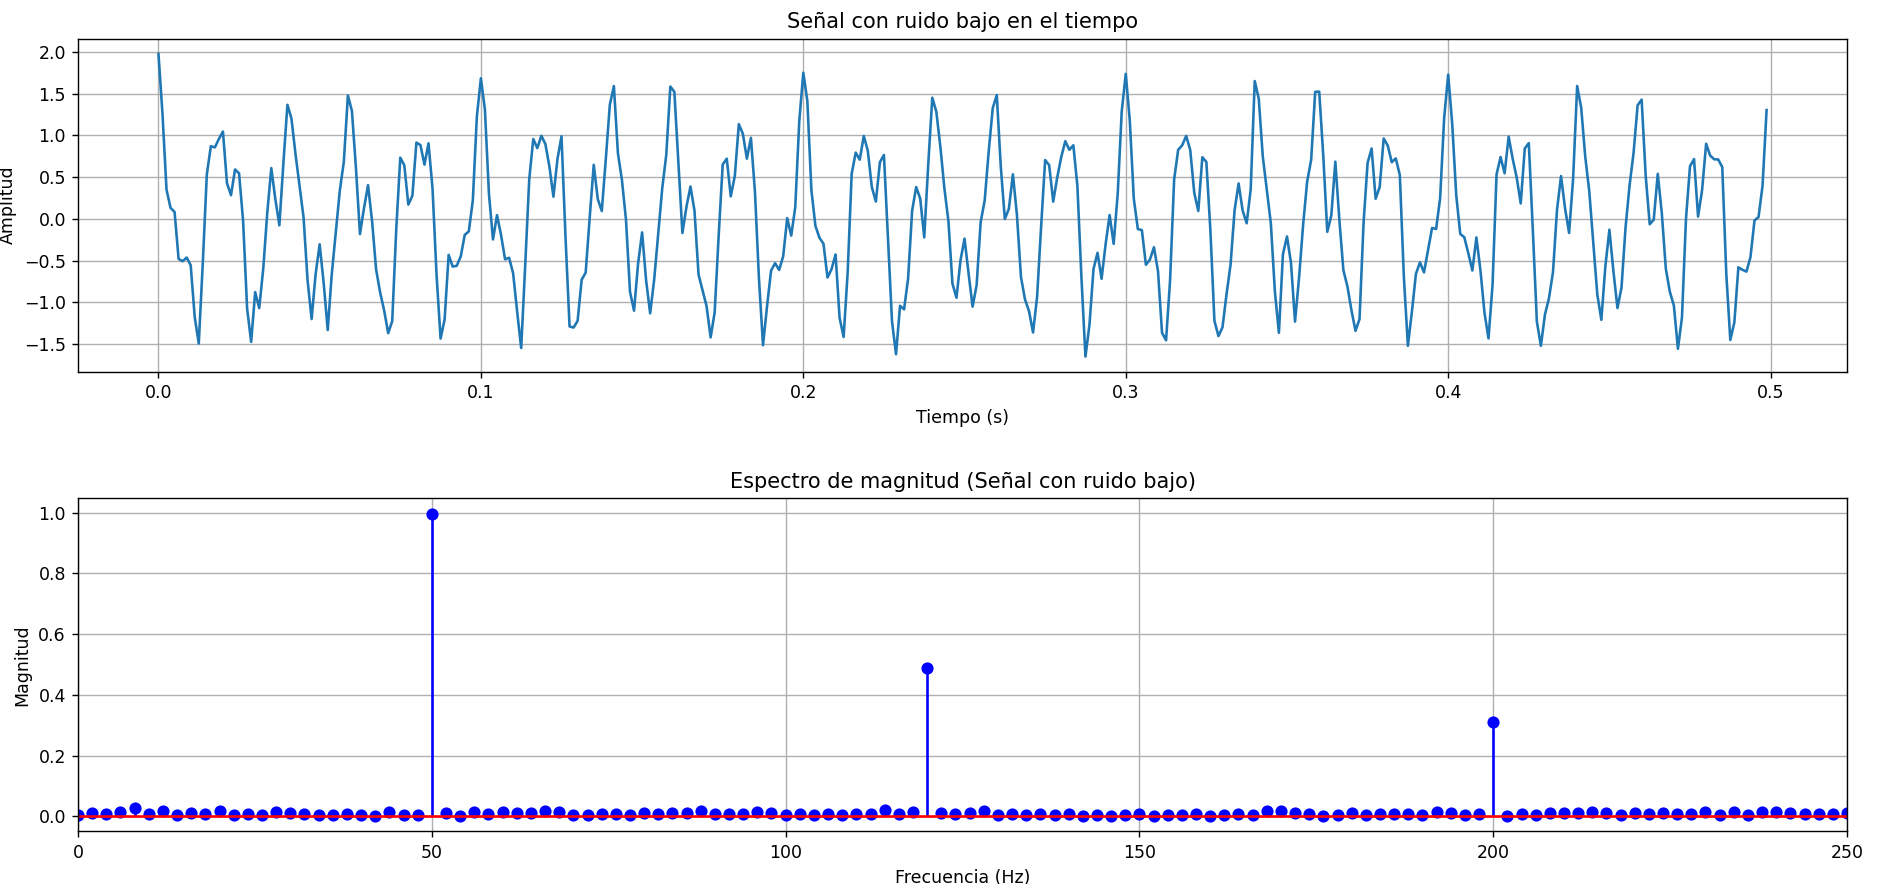
\includegraphics[width=0.8\textwidth]{imagenes/Actividad_5/senalconruidobajo.png}
            \caption{Señal con rudio blanco gaussiano bajo.}
      \end{figure}
\bigskip

\bigskip
      \begin{figure}[H]
            \centering
            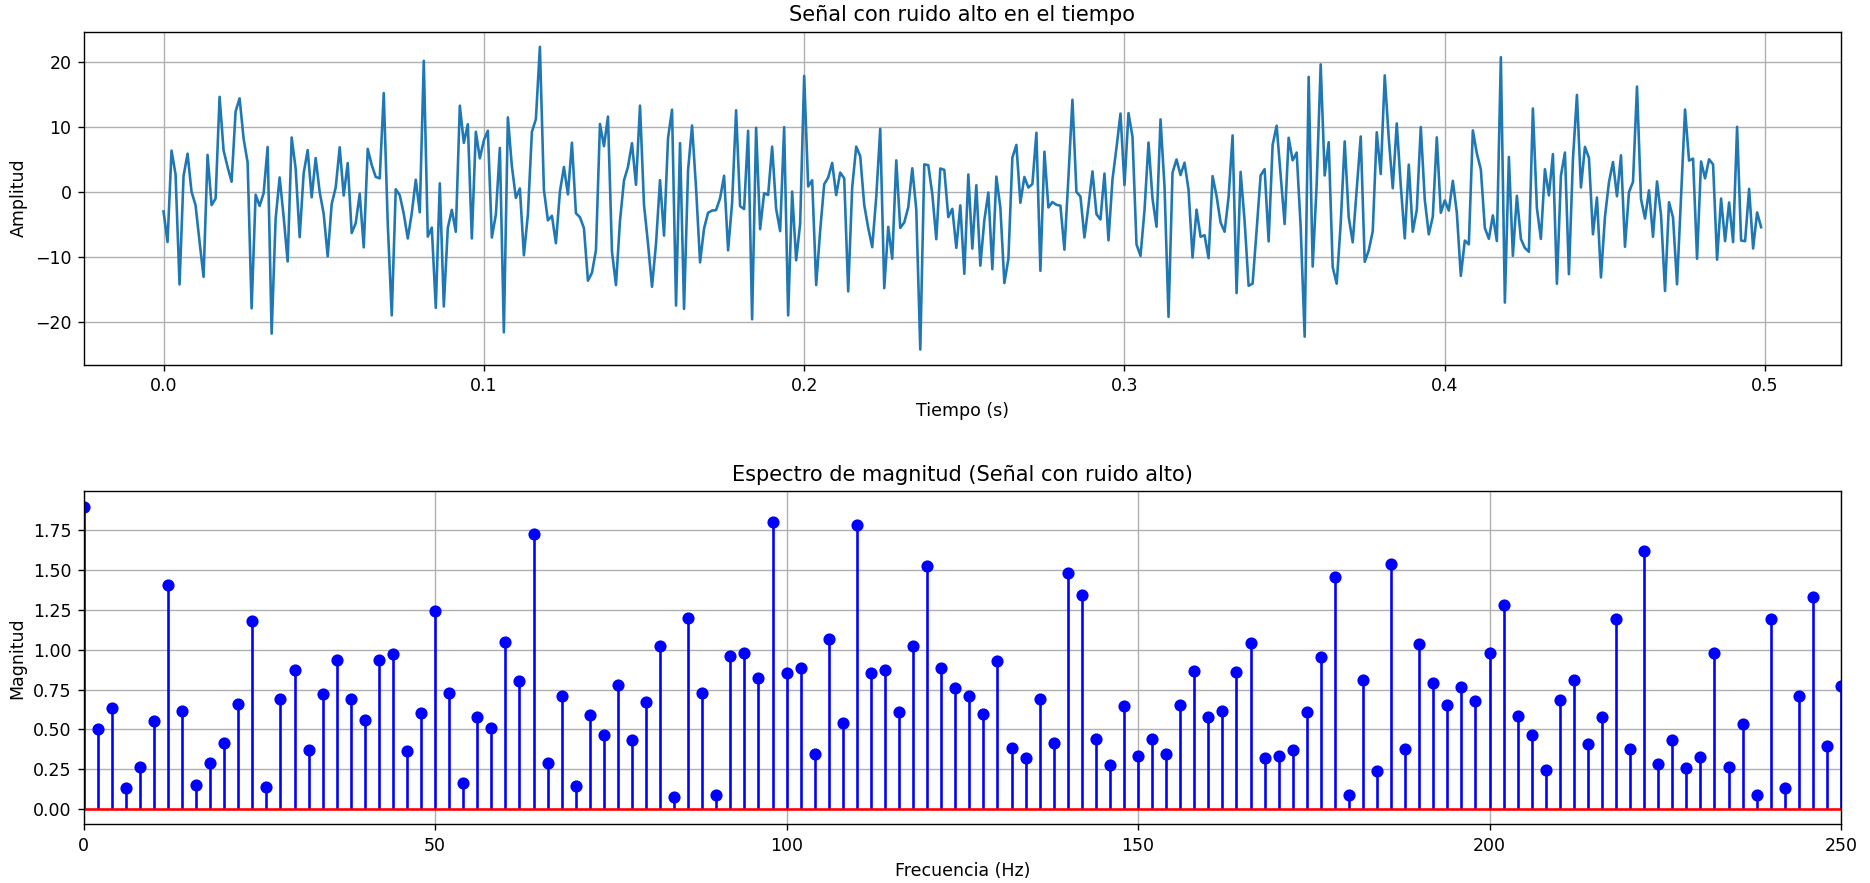
\includegraphics[width=0.8\textwidth]{imagenes/Actividad_5/senalconruidoalto.png}
            \caption{Señal con rudio blanco gaussiano alto.}
      \end{figure}
\bigskip


En las Figuras 5 se observan la gráfica de la señal total con ruido bajo agregado.
\bigskip

Al comparar la señal total con las versiones con ruido, se logra verificar que en el dominio del tiempo la misma no posee ruido, 
presenta una forma suave y definida, mientras que con ruido bajo aparecen pequeñas variaciones sin perder la forma general. Mientras
que con ruido alto la forma original se pierde debido a las variaciones aleatorias. En el dominio de la frecuencia, la señal total sin 
ruido, muestra tres picos en 50 Hz, 120 Hz y 200 Hz, con las frecuencias fuera de las mencionadas en casi cero. Al añadir ruido bajo 
los picos siguen visibles aunque surge un nivel de ruido en todo el espectro (piso de ruido).En cambio, con ruido alto ese piso 
aumenta y los picos se atenúan o se confunden con el ruido. Esto quiere decir que un ruido creciente degrada la forma temporal y 
espectral, dificultando identificar las componentes de la señal original.\par

\bigskip

Por último, se calcula la relación señal-ruido (SNR) para la señal compuesta con amplitudes $A_1=1.0$, $A_2=0.5$ y $A_3=0.3$. 
La potencia media de la señal compuesta se calcula como $A_i^2/2$.

El ruido añadido es blanco y gaussiano con media cero y desviación estándar $\sigma$, por lo que su potencia es $\sigma^2$. 
La relación señal-ruido en decibelios se calcula mediante 
$\text{SNR}_{\mathrm{dB}}=10\log_{10}\!\bigl(P_{\text{señal}}/P_{\text{ruido}}\bigr)$. 
Para el caso de ruido bajo se obtiene un SNR elevado, lo que implica que las componentes espectrales son claramente visibles, 
mientras que para el caso de ruido alto la potencia de ruido domina a la de la señal y se difuculta identificar las componentes de 
la señal total.
\bigskip

\noindent \[
      P_{\text{señal}} = 
      \frac{A_1^2}{2}+\frac{A_2^2}{2}+\frac{A_3^2}{2}=
      \frac{1^2+0.5^2+0.3^2}{2}=
      \frac{1+0.25+0.09}{2}=0.67
\]

\noindent \[
      P_{\text{ruidobajo}}=\sigma_{\text{bajo}}^2=0.1^2=0.01
      \quad\text{y}\quad
      P_{\text{ruidoalto}}=\sigma_{\text{alto}}^2=8^2=64
\]

\noindent \[
      \text{SNR}_{\text{bajo}}=
      10\log_{10}\!\left(\frac{0.67}{0.01}\right)=10\log_{10}(67)=18.3~\text{dB}
\]

\noindent \[
      \text{SNR}_{\text{alto}}=
      10\log_{10}\!\left(\frac{0.67}{64}\right)=10\log_{10}(0.01047)=-19.8~\text{dB}
\]
